\documentclass{beamer}
\usetheme{Boadilla}
\usepackage{graphicx}


\newcommand{\R}{\mathbb{R}}
\newcommand{\ubar}[1]{\underaccent{\bar}{#1}}
\newcommand{\Int}{\text{Int}}
\newcommand{\xbf}{\mathbf{x}}
\newcommand{\Abf}{\mathbf{A}}
\newcommand{\Bbf}{\mathbf{B}}
\newcommand{\Gbf}{\mathbf{G}}
\newcommand{\bbf}{\mathbf{b}}
\newcommand{\Lfn}{\mathcal{L}}
\newcommand{\one}{\mathbbm{1}}

\title[Goldstein et al. ``On ESG Investing"]{\textit{On ESG Investing: Heterogeneous Preferences, Information, and Asset Prices} \\ Itay Goldstein, Alexandr Kopytov, Lin Shen, \\Haotian Xiang \\WP 2022}
\author{Alex von Hafften}
\institute{UW-Madison}

\begin{document}

\section{Introduction}

\begin{frame}
\titlepage
\end{frame}

\begin{frame}
\frametitle{Main Question}
\begin{itemize}[<+->]
\item Environmental, social, and governance (ESG) growing in finance
\begin{itemize}[<+->]
\item In 2014, \$6.6 trillion of ESG-related assets under management
\item In 2020, up to \$17.1 trillion out of \$48.6 trillion total
\end{itemize}
\bigskip
\item Classic paradigm:
\begin{itemize}[<+->]
\item Financial markets aggregate information about fundamentals
\item Price informativeness $\implies$ cost of capital $\implies$ allocation of capital
\item Assumes uniform objectives across investors
\end{itemize}
\bigskip
\item Questions:
\begin{itemize}[<+->]
\item How do asset prices form when investors value assets differently?
\item How to interpret asset prices? What info is incorporated in the price?
\item What are the implications of recent trends?
\end{itemize}
\end{itemize}
\end{frame}


\begin{frame}
\frametitle{Approach}
\begin{itemize}[<+->]
\item A noisy rational expectations equilibrium model \`a la Hellwig (1980)
\bigskip
\item Asset payoff has two risky payoff components:
\begin{itemize}[<+->]
\item Financial cashflow 
\item ESG component
\end{itemize}
\bigskip
\item Two types of risk-averse investors with heterogenous signals:
\begin{itemize}[<+->]
\item Traditional investors ($t$) care only about financial cashflow
\item Green investors ($g$) care about both components
\end{itemize}
\end{itemize}
\end{frame}



\begin{frame}
\frametitle{Main Findings}
\begin{itemize}[<+->]
\item Green and traditional investors trade differently based on same info
\bigskip
\item Multiple equilibria from feedback loop (with low noise):
\begin{itemize}[<+->]
\item Type $i$ dominate $\implies$ price is more informative for $i$ $\implies$ $i$ trade more
\end{itemize}
\bigskip
\item Increase in green investor might increase the cost of capital
\begin{itemize}[<+->]
\item More $g$ investors $\implies$ price comoves more with ESG component $\implies$ price less informative about cash flows and noisier to $t$ investors
\end{itemize}
\bigskip
\item Improved ESG information might indirectly increase cost of capital
\begin{itemize}[<+->]
\item All investors benefit directly from better ESG info, but $g$ investors more
\item $g$ investors trade more $\implies$ price less informative to $t$ investors
\end{itemize}
\end{itemize}
\end{frame}

\AtBeginSection[ ]
{
\begin{frame}{Outline}
    \tableofcontents[currentsection]
\end{frame}
}

\section{Simplified Model}

\begin{frame}
\frametitle{Environment - Assets}
\begin{itemize}[<+->]
\item Unlimited supply of risk-free asset
\begin{itemize}[<+->]
\item Payoff and price normalized to one
\end{itemize}
\bigskip
\item Unit supply of risky asset, ``stock"
\begin{itemize}[<+->]
\item $\tilde z$ is monetary factor in payoff and $\tilde \delta$ is non-monetary factor in payoff
$$
\tilde z, \tilde \delta \sim_{iid} N(0, \tau^{-1})
$$
\item Price $\tilde p$ is determined by market clearing
\end{itemize}
\end{itemize}
\end{frame}



\begin{frame}
\frametitle{Environment - Market Participants}
\begin{itemize}[<+->]
\item Rational investors trade on signals and learn from price
\begin{itemize}[<+->]
\item Traditional ($\beta_z^t = 1$ and $\beta_\delta^t = 0$) and green ($\beta_z^g = 0$ and $\beta_\delta^g = 1$)
\item Mass of each group is $\frac{m}{2}$
\item Investor $i$ of type $j$ holding $d_j^i$ shares has CARA expected utility
$$
E\{ - \exp (-\gamma [W_0^i + d_j^i(\tilde v_j - \tilde q])\}
$$
where $\tilde v_j = \beta_z^j \tilde z + \beta_\delta^j \tilde \delta$ is per-unit payoff
\item Each investor receives private signals about each factor
$$
\tilde s^i_z \sim_{iid} N(\tilde z, \tau_s^{-1}), \tilde s^i_\delta \sim_{iid} N(\tilde \delta, \tau_s^{-1})
$$
\item Define info set $\mathcal{F}_i \equiv \{\tilde s^i_z, \tilde s^i_\delta, \tilde p\}$ of investor $i$
\end{itemize}
\bigskip
\item Noise traders
\begin{itemize}[<+->]
\item Demand is $\tilde N(0, \tau_n^{-1})$
\end{itemize}
\end{itemize}
\end{frame}



\begin{frame}
\frametitle{Market Clearing}
\begin{itemize}[<+->]
\item Market clearing

$$
\underbrace{D_t(\tilde z, \tilde \delta, \tilde p)}_{\equiv \int_{i \in \mathcal{T}_t} d_t^i(\mathcal{F}_i)di} + \underbrace{D_g(\tilde z, \tilde \delta, \tilde p)}_{\equiv \int_{i \in \mathcal{T}_g} d_g^i(\mathcal{F}_i) di} + \tilde n = 1
$$

\bigskip

\item Focus on equilibria with linear prices

\begin{align*}
\tilde p 
&= p_0 + p_z \tilde z + p_\delta \tilde \delta + p_n \tilde n \\
&= p_0 + p_n(\xi_z \tilde z + \xi_\delta \tilde \delta + \tilde n) 
\end{align*}

where $\xi_z \equiv \frac{q_z}{q_n}$ and  $\xi_\delta \equiv \frac{q_\delta}{q_n}$ is normalized price coefficeint


\end{itemize}
\end{frame}

\begin{frame}
\frametitle{Trading Intensity}
\begin{itemize}[<+->]
\item CARA utility $\implies$ traditional investor demand
$$
d_t(\mathcal{F}) 
=
\frac{1}{\gamma} 
\frac{E[\tilde z | \mathcal{F}] - \tilde p}{V[\tilde z | \mathcal{F}]}
$$
where 
\begin{align*}
E[\tilde z | \mathcal{F}] 
&= 
\underbrace{\tilde s_z \frac{\tau_s}{\tau_s + \tau}}_{\text{inference from private signal}}\\
&+ 
\underbrace{\frac{\xi_z \frac{1}{\tau + \tau_s}[\tilde p/ p_n - (p_0/p_n + \xi_z \tilde s_z \frac{\tau_s}{\tau_s + \tau} + \xi_\delta \tilde s_\delta \frac{\tau_s}{\tau_s + \tau})]}{\xi_z^2 \frac{1}{\tau + \tau_s} + \xi_\delta^2 \frac{1}{\tau + \tau_s} + \frac{1}{\tau_n}}}_{\text{inference from the price}}
\end{align*}

\item $\tilde s_\delta$ is not informative about $\tilde z$, but has price inference effect

\end{itemize}
\end{frame}


\begin{frame}
\frametitle{Trading Intensity}
\begin{itemize}[<+->]
\item \textit{Trading intensity} is the change in demand given change in signal

\bigskip

\item For traditional investor,

\begin{align*}
i_t^z &\equiv \frac{\partial d^t}{\partial \tilde s_z} = \frac{\tau_s}{\gamma} > 0\\
i_t^\delta &\equiv \frac{\partial d^t}{\partial \tilde s_\delta} = -\frac{\tau_s}{\gamma} \frac{\overbrace{\xi_\delta \xi_z}^{\text{Strength of inference}}}{ \underbrace{\xi_\delta^2 + \frac{\tau + \tau_s}{\tau_n}}_{\text{price noisiness}}} < 0
\end{align*}

\item Opposite for green investor $i_g^z < 0$ and $i_g^\delta > 0$

\bigskip

\item Constant trading intensity for signal about valued factor

\end{itemize}
\end{frame}


\begin{frame}
\frametitle{Feedback Loop}
\begin{itemize}[<+->]
\item How actively do investor trade on signals about non-valued factor?
$$
\frac{i_t^\delta}{i_g^z} = \frac{\xi_z^2 + \frac{\tau + \tau_s}{\tau_n}}{\xi_\delta^2 + \frac{\tau + \tau_s}{\tau_n}} = \frac{PI_t}{PI_g}
$$

where $PI_j \equiv [V(\tilde v_j | \mathcal{F})]^{-1}$ is the \textit{price informativeness} for type $j$

\bigskip

\item Feedback loop

\begin{itemize}[<+->]

\item $\frac{PI_t}{PI_g}$ is high $\implies$ traditional investors dominate trading $\implies$ price is informative about $\tilde z$ but not $\tilde \delta$ $\implies$ $\frac{PI_t}{PI_g}$ is high
\item $\frac{PI_t}{PI_g}$ is low $\implies$ green investors dominate trading $\implies$ price is informative about $\tilde \delta$ but not $\tilde z$ $\implies$ $\frac{PI_t}{PI_g}$ is low

\end{itemize}

\bigskip

\item Feedback is strong when noise is small

\begin{itemize}[<+->]

\item Large noise $\implies \frac{i_t^\delta}{i_g^z}\to 1$ as $\tau_n^{-1} \to \infty \implies$ uninformative price 

\item Small noise $\implies \frac{i_t^\delta}{i_g^z}\to \frac{\xi_z^2}{\xi_\delta^2}$ as $\tau_n^{-1} \to 0 \implies$ strong feedback loop

\end{itemize}

\end{itemize}
\end{frame}



\begin{frame}
\frametitle{Multiple Equilibria}
\begin{itemize}[<+->]
\item Trading intensity determine price coefficients:
\begin{align*}
\xi_z &= \frac{m}{2}i_g^z + \frac{m}{2}i_t^z = \frac{m}{2} \frac{\tau_s}{\gamma} \Bigg[1 - \frac{\xi_z \xi_\delta}{\xi_z^2 + \frac{\tau +\tau_s}{\tau_n}}\Bigg]\\
\xi_\delta &= \frac{m}{2}i_g^\delta + \frac{m}{2}i_t^\delta = \frac{m}{2} \frac{\tau_s}{\gamma} \Bigg[1 - \frac{\xi_z \xi_\delta}{\xi_\delta^2 + \frac{\tau +\tau_s}{\tau_n}}\Bigg]
\end{align*}
\bigskip
\item Exists a noise threshold $\hat{\tau}_n = 4(\tau + \tau_s) (\frac{\tau_2}{\gamma}\frac{m}{2})^{-2}$
\bigskip
\item  Large noise $\tau_n^{-1} \ge \hat\tau_n^{-1} \implies$ unique equilibrium with $\xi_z = \xi_\delta$
\bigskip
\item Small noise $\tau_n^{-1} < \hat\tau_n^{-1} \implies$ three equilibria
\begin{itemize}[<+->]
\item Stable T-equilibrium with $\xi_z > \xi_\delta$ and $PI_t > PI_g$
\item Stable G-equilibrium with $\xi_z < \xi_\delta$ and $PI_t < PI_g$
\item Unstable M-equilibrium with $\xi_z = \xi_\delta$ and $PI_t = PI_g$
\end{itemize}
\end{itemize}
\end{frame}


\begin{frame}
\frametitle{Multiple Equilibria}
\begin{center}
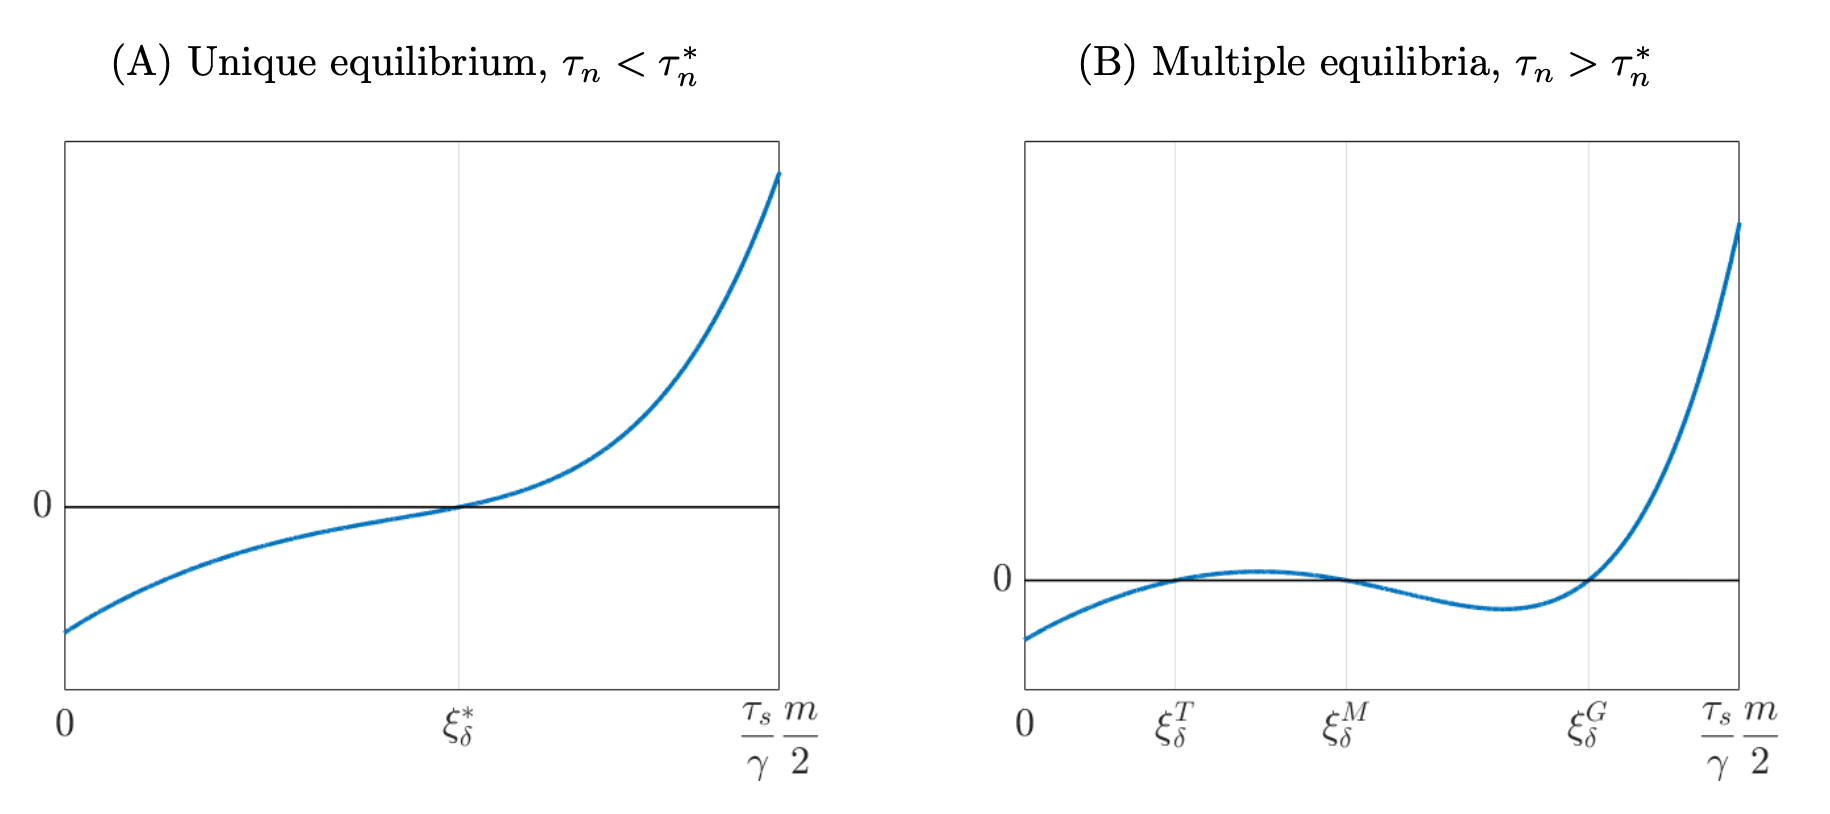
\includegraphics[scale=0.35]{multiple_equilibria}
\end{center}
Unique equilibrium with small noise and multiple equilibria with large noise
\end{frame}



\section{Other Findings}

\begin{frame}
\frametitle{Baseline Model}
\begin{itemize}[<+->]
\item Generalization:
\begin{itemize}[<+->]
\item Allow green investors to care about both components of payoff
\item Unequal masses of investors
\item Index equilibria by signal precision
\item Dependence between $\tilde\delta$ and $\tilde z$
\end{itemize}
\bigskip
\item Consider the cost of capital:
$$
CoC = E[\tilde z - \tilde p] = \frac{\gamma}{m_t PI_t + m_g PI_g}
$$
\item How does cost of capital change with more green investors?
\bigskip
\item How does cost of capital change with better info about $\tilde\delta$?
\end{itemize}
\end{frame}


\begin{frame}
\frametitle{Cost of Capital with More Green Investors}
\begin{center}
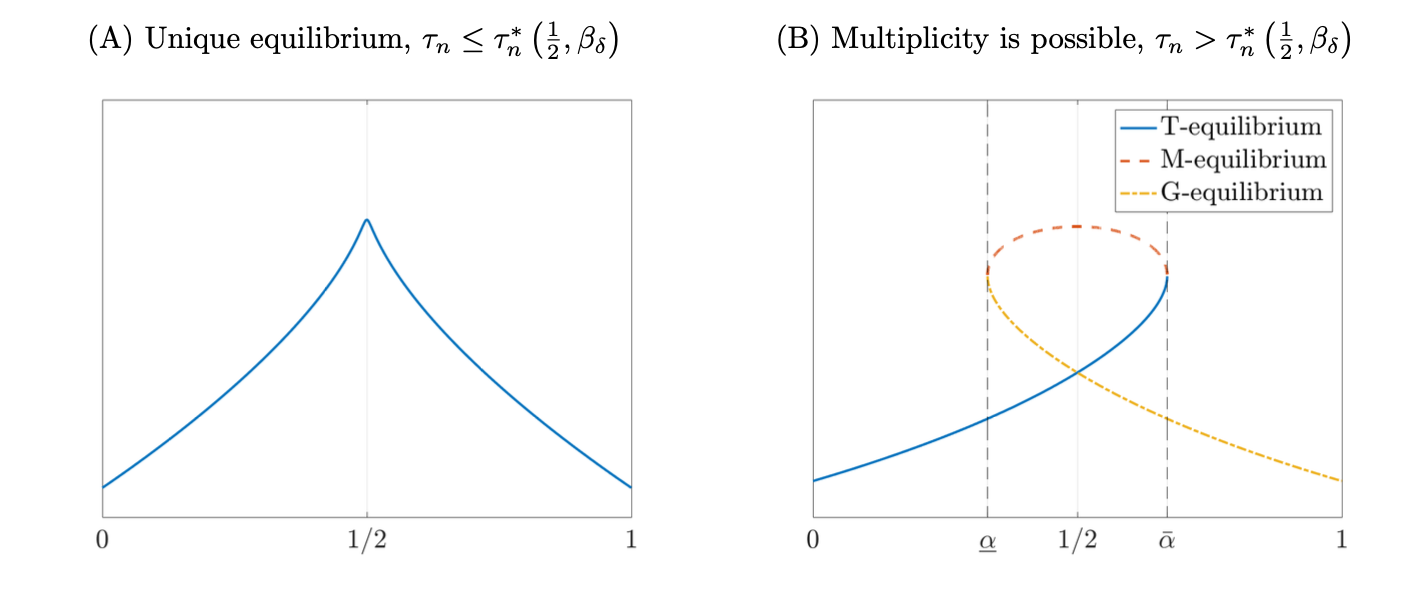
\includegraphics[scale=0.5]{investor_share}
\end{center}
\begin{itemize}[<+->]
\item $\alpha$ is fraction of green investors
\item Cost of capital is highest when investor base is balanced
\end{itemize}
\end{frame}

\begin{frame}
\frametitle{Cost of Capital with More Precise ESG Signals}
\begin{center}
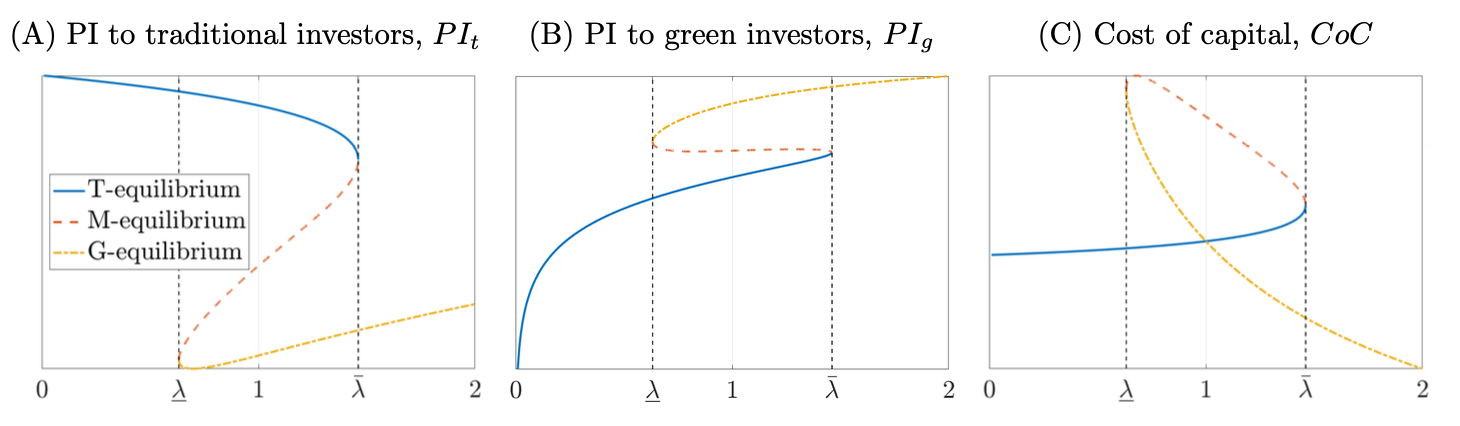
\includegraphics[scale=0.45]{information}
\end{center}
\begin{itemize}[<+->]
\item $\lambda$ indexes precision of signals about $\delta$ (high $\lambda$ is more precision)
\item Direct effect: $\lambda \uparrow \implies PI_t \uparrow$ and $PI_g \uparrow\uparrow\uparrow$
\item Indirect effect: $\lambda \uparrow \implies i_g^\delta \uparrow \implies PI_t \downarrow$
\end{itemize}
\end{frame}

\section{Conclusion and Discussion}

\begin{frame}
\frametitle{Conclusion}
\begin{itemize}[<+->]
\item REE model with investors with heterogenous valuations
\begin{itemize}[<+->]
\item Contribution: Combine (1) heterogeneous preferences over multiple fundamentals and (2) info sets with signals about all fundamentals
\end{itemize}
\bigskip
\item Show how investor base matters $\implies$ May reconcile mixed evidence on green premium/discount
\bigskip
\item Novel channel for better ESG-disclosures to backfire
\end{itemize}
\end{frame}


\begin{frame}
\frametitle{Discussion - Green Investor Preferences}
\begin{itemize}[<+->]
\item In the paper, green investors prefer for ESG factor is like consumption
\bigskip
\item Unclear if this form of preferences is consistent with other research
\bigskip
\item Using an experimental approach, Heeb et al (2021) find that green investors have a higher WTP for a sustainable investment, but their WTP does not grow with the social impact of the investment
\end{itemize}
\end{frame}





\begin{frame}
\frametitle{Discussion - Endogenous Information Acquisition}
\begin{itemize}[<+->]
\item In the paper, signals are exogenous processes
\bigskip
\item In appendix, they do allow for correlated signals
\bigskip
\item How would endogenous information acquisition affect results?
\bigskip
\item Green investors have direct incentive to discover info about ESG
\bigskip
\item But do traditional investors really have private signals about ESG?
\bigskip
\item Seems less plausible that traditional investors seek to acquire information about ESG impacts to better trade against green investors
\end{itemize}
\end{frame}

\begin{frame}
\frametitle{Discussion - Other}
\begin{itemize}[<+->]
\item Testing this model's implications is challenging due to issues measuring ESG impacts (i.e. Allcott et al 2021, Berg et al 2021)
\bigskip
\item More detailed ESG disclosures themselves may increase $\tilde\delta$. Kreuger et al (2021) found that firms who were required to disclose more detailed information about ESG-related issue had fewer negative ESG-related incidents (i.e. chemical spills)
\end{itemize}
\end{frame}



\end{document}

